\subsection{Kalibrierung der kleinen Scheibe}
Für die kleine Drehscheibe wurden alle $\unit[45]{^\circ}$ die resultierende Kraft bei einem Radius $r = \unit[(18.8 \pm 0.3)]{cm}$ gemessen (siehe Abbildung \ref{fig:kal1}). Mit linearer Regression\footnote{Berechnung durch Origin} bekommen wir eine Steigung von $d = \unit[(23.9 \pm 0.1)]{mN m}$.\\
Zudem kann die Winkelrichtgröße durch die Steigung ermittelt werden. Durch Formel \ref{eq:wink}:
\begin{equation}
T^2 = \frac{4\pi^2}{d}\cdot (J_0+J_Z)
\end{equation}
Der y-Achsenabschnitt $f = \unit[(0.57 \pm 0.06)]{s^2}$ ergibt sich durch die Regression, und somit ist $J_0$
\begin{align}
J_0 &= f^2\frac{d}{4\pi^2}\\
J_0 &= \unit[183.8 \pm 1.2]{g m^2}
\end{align}
Somit können wir $d$ berechnen:
\begin{equation*}
d = \frac{4\pi^2}{W} = \unit[(22.33 \pm 0.3)]{mN cm}
\end{equation*}


\begin{figure}
\begin{center}
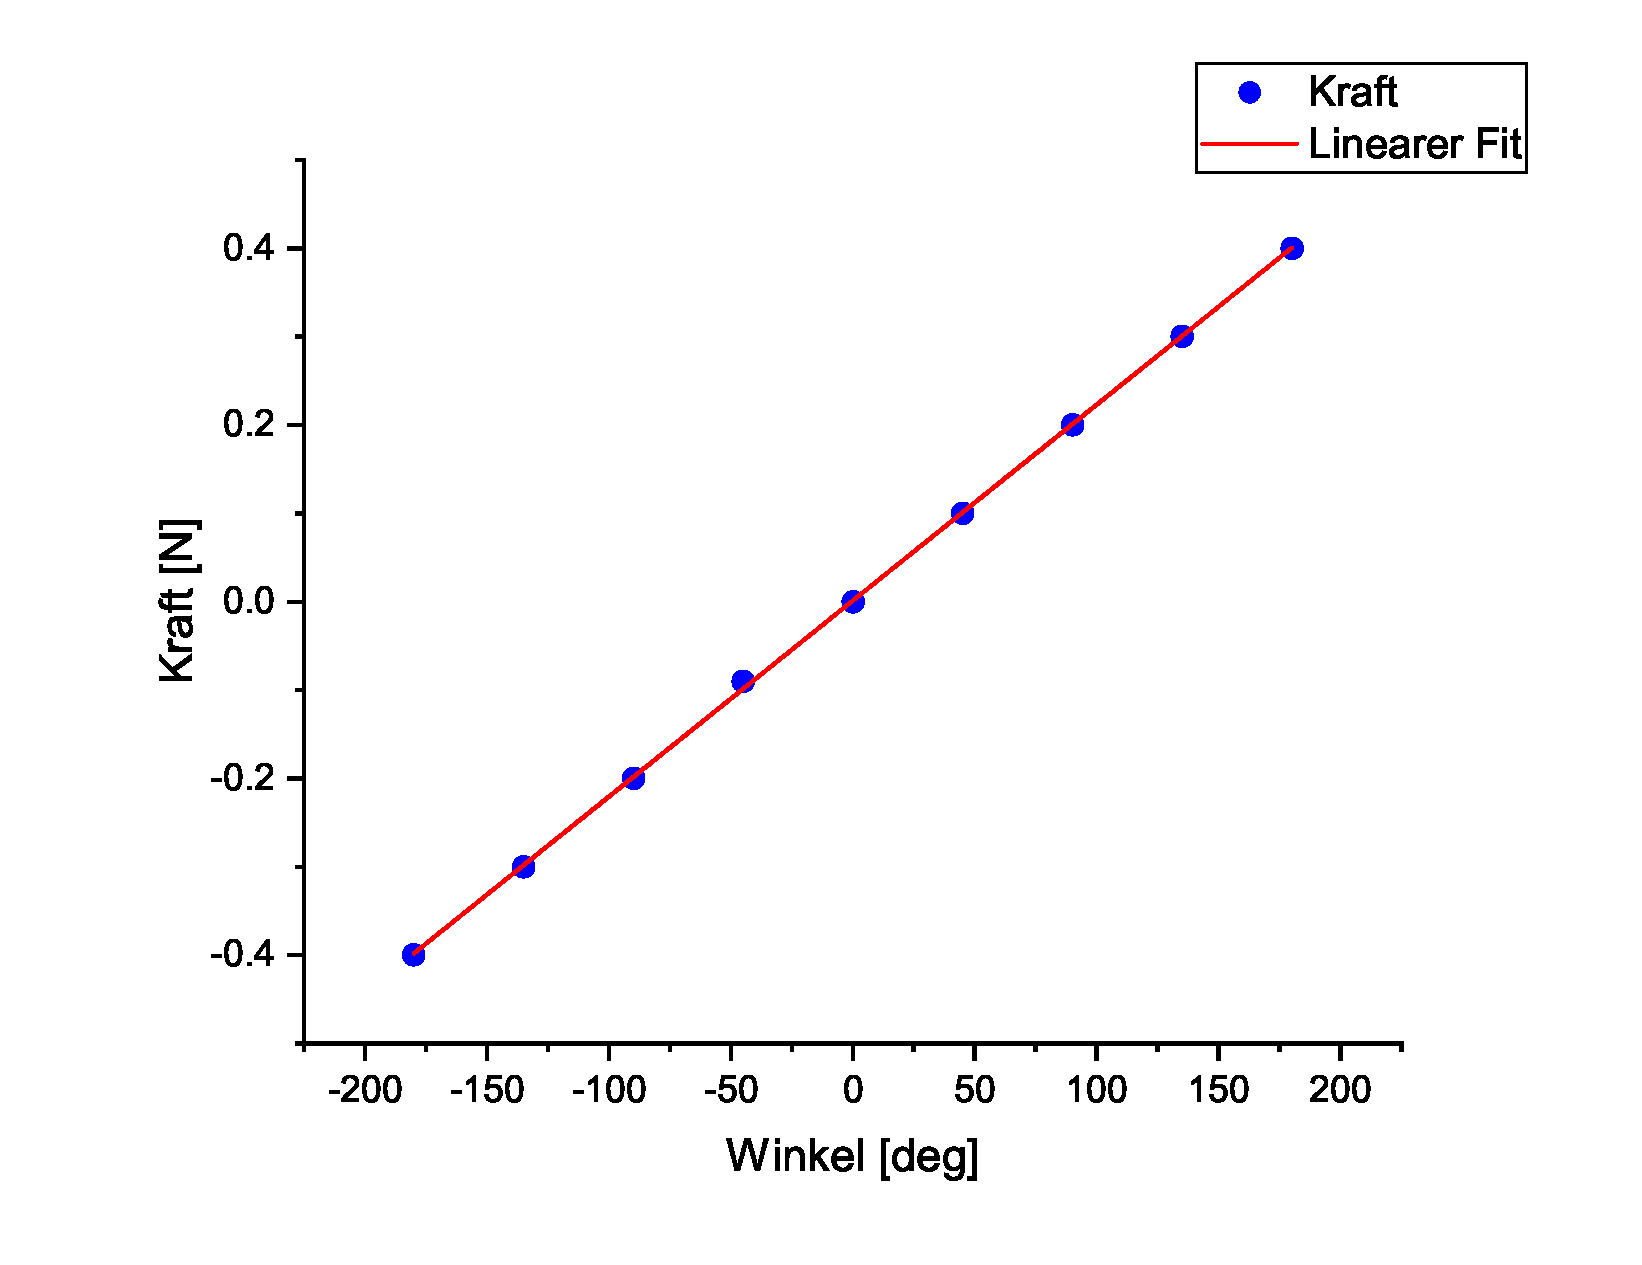
\includegraphics[width=0.7\textwidth]{Bilder/kal1.eps}
\caption{Kalibrierung der kleinen Scheibe}
\label{fig:kal1}
\end{center}
\end{figure}
